\documentclass[12pt]{article}

\usepackage{fullpage}
\usepackage{multicol,multirow}
\usepackage{tabularx}
\usepackage{ulem}
\usepackage[utf8]{inputenc}
\usepackage[russian]{babel}
\usepackage{amsmath}
\usepackage{amssymb}

\usepackage{graphicx}
\DeclareGraphicsExtensions{.png}

\usepackage{titlesec}

\titleformat{\section}
  {\normalfont\Large\bfseries}{\thesection.}{0.3em}{}

\titleformat{\subsection}
  {\normalfont\large\bfseries}{\thesubsection.}{0.3em}{}

\titlespacing{\section}{0pt}{*2}{*2}
\titlespacing{\subsection}{0pt}{*1}{*1}
\titlespacing{\subsubsection}{0pt}{*0}{*0}
\usepackage{listings}
\lstloadlanguages{Lisp}
\lstset{extendedchars=false,
    breaklines=true,
    breakatwhitespace=true,
    keepspaces = true,
    tabsize=2
}
\begin{document}


\section*{Отчет по лабораторной работе №\,3
по курсу \guillemotleft  Функциональное программирование\guillemotright}
\begin{flushright}
Студентка группы М8О-307 МАИ \textit{Довженко Анастасия}, \textnumero 7 по списку \\
\makebox[7cm]{Контакты: {\tt tutkarma@gmail.com} \hfill} \\
\makebox[7cm]{Работа выполнена: 23.03.2019 \hfill} \\
\ \\
Преподаватель: Иванов Дмитрий Анатольевич, доц. каф. 806 \\
\makebox[7cm]{Отчет сдан: \hfill} \\
\makebox[7cm]{Итоговая оценка: \hfill} \\
\makebox[7cm]{Подпись преподавателя: \hfill} \\

\end{flushright}

\section{Тема работы}
Последовательности, массивы и управляющие конструкции Common Lisp.

\section{Цель работы}
Научиться создавать векторы и массивы для представления матриц, освоить общие функции работы с последовательностями, инструкции цикла и нелокального выхода.

\section{Задание (вариант №3.42)}
Запрограммировать на языке Коммон Лисп функцию, принимающую в качестве единственного аргумента целое число {\tt n} - порядок матрицы. Функция должна создавать и возвращать двумерный массив, представляющий целочисленную квадратную матрицу порядка {\tt n}, элементами которой являются числа {\tt $1, 2, ... n^{2}$}, расположенные по схеме, показанной на рисунке.

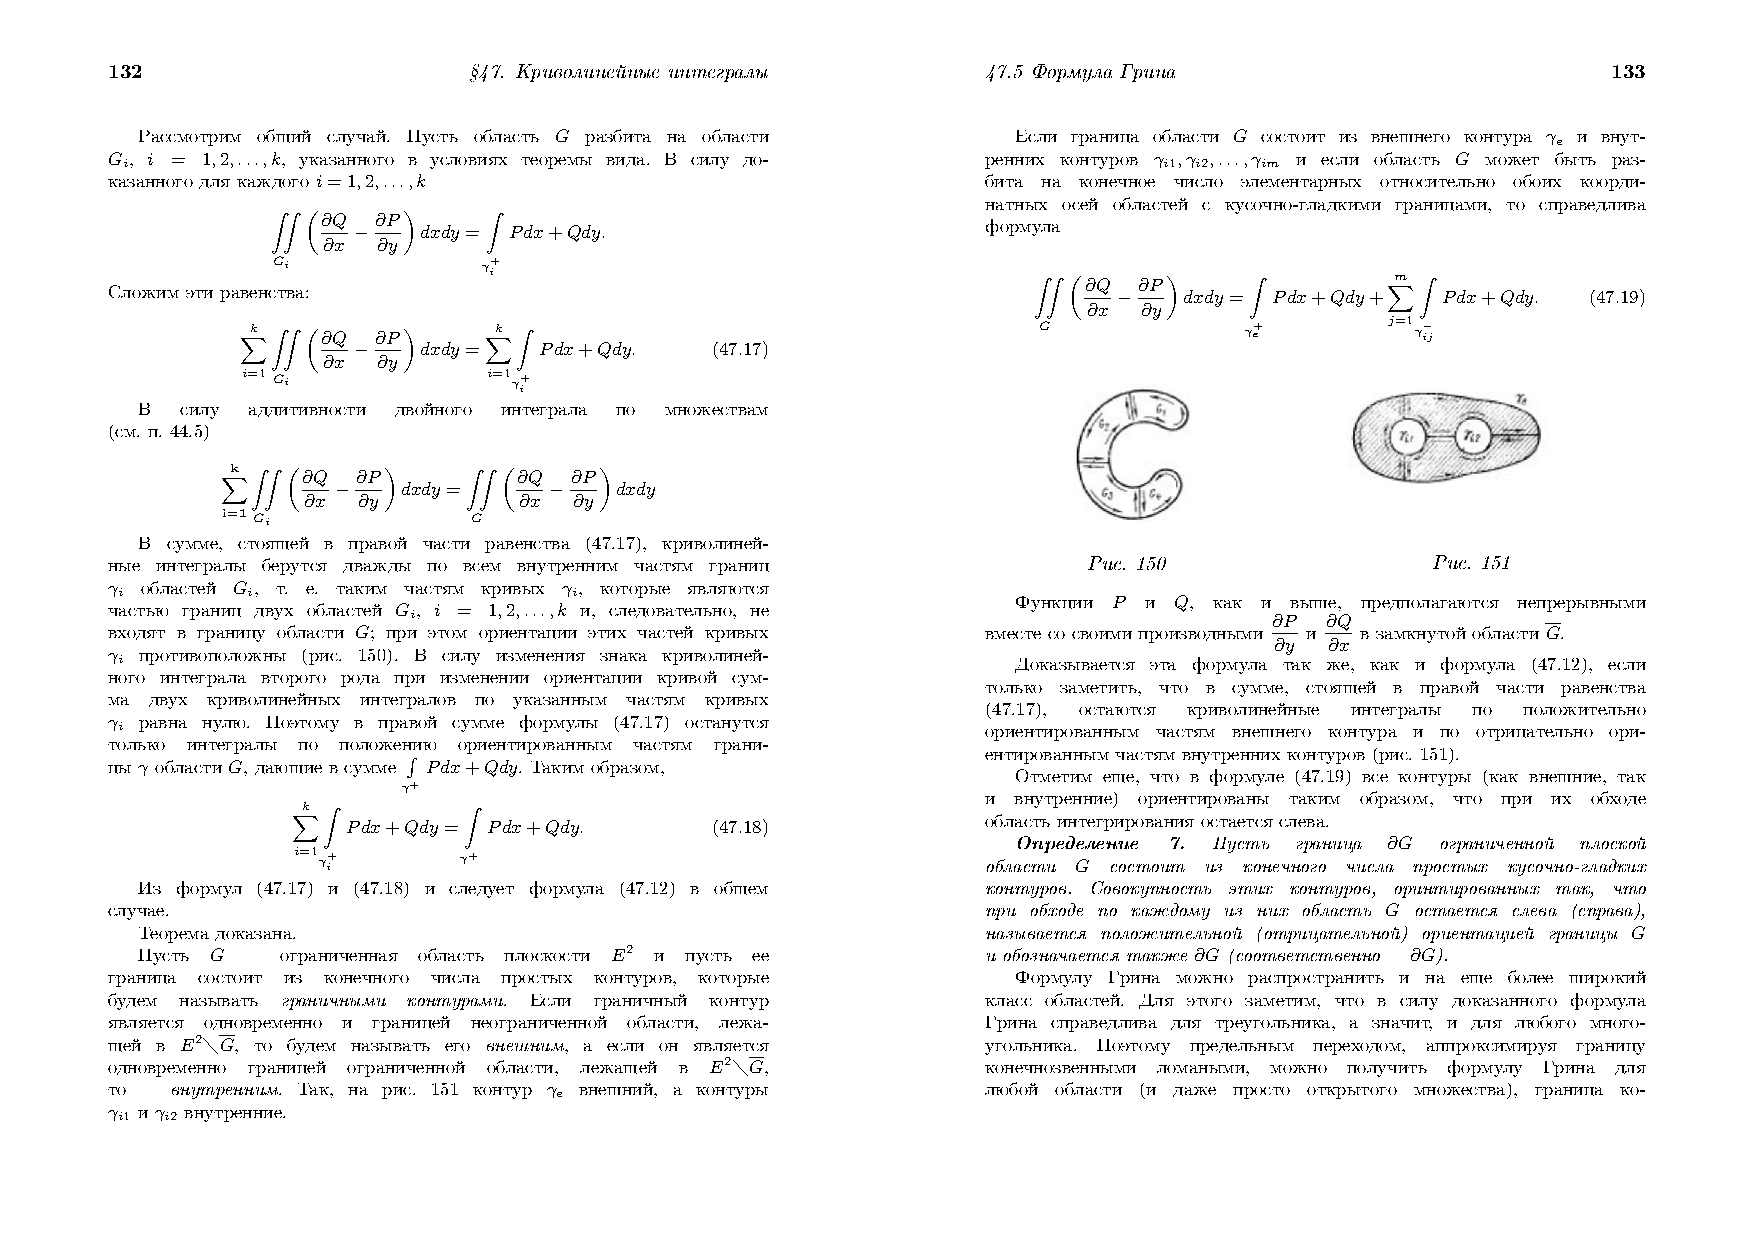
\includegraphics{1.png}

\section{Оборудование студента}
Ноутбук Asus UX310U, процессор Intel Core i7-6500U CPU 2.50GHz x 4, память: 8Gb, разрядность системы: 64.

\section{Программное обеспечение}
ОС Ubuntu 16.04 LTS, компилятор clisp, текстовый редактор Sublime Text 3.

\section{Идея, метод, алгоритм}
Заполняем матрицу постолбцово, причем четные столбцы заполняются сверху вниз, а нечетные -- снизу вверх. При каждом заполнении увеличиваем локальный счетчик на единицу, что позволяет выполнить условие, при котором элементами матрицы являюся числа от единицы до квадрата исходного числа {\tt n}. На каждом шаге цикла заполняются два столбца -- четный и нечетный. Если исходное число {\tt n} -- нечетное, то последний нечетный столбец не заполняется, потому что его нет.

\section{Сценарий выполнения работы}

\section{Распечатка программы и её результаты}

\subsection{Исходный код}
\lstinputlisting{./main.lisp}

\subsection{Результаты работы}
\begin{lstlisting}
#2A((1)) 
#2A((1 10 11 20 21)
    (2 9 12 19 22)
    (3 8 13 18 23)
    (4 7 14 17 24)
    (5 6 15 16 25)) 
#2A((1 16 17 32 33 48 49 64)
    (2 15 18 31 34 47 50 63)
    (3 14 19 30 35 46 51 62)
    (4 13 20 29 36 45 52 61)
    (5 12 21 28 37 44 53 60)
    (6 11 22 27 38 43 54 59)
    (7 10 23 26 39 42 55 58)
    (8 9 24 25 40 41 56 57))
\end{lstlisting}

\section{Дневник отладки}
\begin{tabular}{|p{50pt}|p{130pt}|p{130pt}|p{70pt}|}
\hline
Дата & Событие & Действие по исправлению & Примечание\\
\hline
\end{tabular}

\section{Замечания автора по существу работы}
Я уже встечалась с подобной задачей обхода матрицы в одной из лабораторных на 1 курсе, поэтому алгоритмически она не показалась мне сложной, зато было интересно сравнить реализации двух разных парадигм. 

\section{Выводы}
Я познакомилась с массивами в языке Lisp, а также узнала, как выполнять различные операции над ними, как использовать циклы. Массивы являются основополагающей структурой данных в программировании и часто используются, потому что в них удобно хранить данные. Для языка Lisp существуют целые библиотеки для работы с матрицами, может быть когда-нибудь я напишу свою, всякое может случиться, никогда не знаешь, что тебе пригодится в будущем.
\end{document}